\documentclass[11pt]{article}
\usepackage[utf8]{inputenc}\usepackage[T1]{fontenc}\usepackage{lmodern}
\usepackage[a4paper,margin=1in,headheight=14pt]{geometry}
\usepackage{graphicx}\usepackage{booktabs}\usepackage{amsmath,amssymb,amsthm,mathtools,bm}
\usepackage{siunitx}\usepackage{caption}\usepackage{microtype}
\usepackage[numbers,sort&compress]{natbib}
\usepackage{xcolor}\definecolor{nmiaccent}{HTML}{1A4E8A}
\usepackage[colorlinks=true,allcolors=nmiaccent]{hyperref}
\usepackage{titlesec}\usepackage{fancyhdr}\usepackage{authblk}
\captionsetup{font=small,labelfont=bf,labelsep=period}
\graphicspath{{code/figures/}}\setlength{\parskip}{0.45em}\setlength{\emergencystretch}{3em}
\renewcommand{\Affilfont}{\normalsize\itshape}\renewcommand{\Authfont}{\large\bfseries}
\titleformat{\section}{\sffamily\large\bfseries\color{nmiaccent}}{\thesection}{0.6em}{}
\titleformat{\subsection}{\sffamily\normalsize\bfseries}{\thesubsection}{0.6em}{}
\pagestyle{fancy}\fancyhf{}\fancyhead[L]{\footnotesize\itshape Spectral-truncation-kernel QAOA schedule transfer}\fancyhead[R]{\footnotesize\thepage}\renewcommand{\headrulewidth}{0.4pt}

% Convenience macros. \sync{...} is the identity, marking values that originate
% from the generated results. Every numerical value in this manuscript is read
% from auto-generated macros (code/results/macros.tex), so nothing is typed by
% hand; \ket / \expval render QAOA quantities.
\newcommand{\sync}[1]{#1}
\newcommand{\ket}[1]{\left\lvert #1 \right\rangle}
\newcommand{\bra}[1]{\left\langle #1 \right\rvert}
\newcommand{\expval}[1]{\left\langle #1 \right\rangle}
\newcommand{\abs}[1]{\left\lvert #1 \right\rvert}
\newcommand{\norm}[1]{\left\lVert #1 \right\rVert}
% Auto-generated by scripts/make_tables.py -- do not edit by hand.
\newcommand{\Ngraphs}{84}
\newcommand{\Nfamilies}{6}
\newcommand{\budgetval}{28}
\newcommand{\seedval}{0}
\newcommand{\Ndepths}{3}
\newcommand{\headlinedepth}{2}
\newcommand{\stkr}{6}
\newcommand{\sizesval}{8,10,12,14}
\newcommand{\runtimeval}{423.3409}
\newcommand{\peakmem}{163.2}
\newcommand{\leakageclean}{true}
\newcommand{\verPython}{3.9.6}
\newcommand{\verNumpy}{2.0.2}
\newcommand{\verScipy}{1.13.1}
\newcommand{\verNetworkx}{3.2.1}
\newcommand{\verSklearn}{1.6.1}
\newcommand{\verMatplotlib}{3.9.4}
\newcommand{\frRandomPI}{0.7287}
\newcommand{\ciRandomPI}{0.0179}
\newcommand{\fqRandomPI}{0.6186}
\newcommand{\frSpectralPI}{0.7823}
\newcommand{\ciSpectralPI}{0.0111}
\newcommand{\fqSpectralPI}{0.7425}
\newcommand{\frTopologyPI}{0.7825}
\newcommand{\ciTopologyPI}{0.0111}
\newcommand{\fqTopologyPI}{0.7759}
\newcommand{\frGcPI}{0.7824}
\newcommand{\ciGcPI}{0.0111}
\newcommand{\fqGcPI}{0.7452}
\newcommand{\frStkPI}{0.7825}
\newcommand{\ciStkPI}{0.0111}
\newcommand{\fqStkPI}{0.7790}
\newcommand{\oraclePI}{0.7827}
\newcommand{\deltaStkRampPI}{+0.0000}
\newcommand{\ciDeltaStkRampPI}{0.0001}
\newcommand{\deltaStkRampFqPI}{+0.0030}
\newcommand{\deltaStkSpecPI}{+0.0002}
\newcommand{\sigStkRampPI}{no}
\newcommand{\deltaGcRampPI}{-0.0001}
\newcommand{\frRandomPII}{0.7474}
\newcommand{\ciRandomPII}{0.0208}
\newcommand{\fqRandomPII}{0.6057}
\newcommand{\frSpectralPII}{0.8319}
\newcommand{\ciSpectralPII}{0.0095}
\newcommand{\fqSpectralPII}{0.7483}
\newcommand{\frTopologyPII}{0.8394}
\newcommand{\ciTopologyPII}{0.0088}
\newcommand{\fqTopologyPII}{0.8032}
\newcommand{\frGcPII}{0.8470}
\newcommand{\ciGcPII}{0.0080}
\newcommand{\fqGcPII}{0.8050}
\newcommand{\frStkPII}{0.8503}
\newcommand{\ciStkPII}{0.0081}
\newcommand{\fqStkPII}{0.8449}
\newcommand{\oraclePII}{0.8536}
\newcommand{\deltaStkRampPII}{+0.0103}
\newcommand{\ciDeltaStkRampPII}{0.0019}
\newcommand{\deltaStkRampFqPII}{+0.0416}
\newcommand{\deltaStkSpecPII}{+0.0185}
\newcommand{\sigStkRampPII}{yes}
\newcommand{\deltaGcRampPII}{+0.0076}
\newcommand{\frRandomPIII}{0.7469}
\newcommand{\ciRandomPIII}{0.0155}
\newcommand{\fqRandomPIII}{0.6025}
\newcommand{\frSpectralPIII}{0.8568}
\newcommand{\ciSpectralPIII}{0.0073}
\newcommand{\fqSpectralPIII}{0.8129}
\newcommand{\frTopologyPIII}{0.8622}
\newcommand{\ciTopologyPIII}{0.0064}
\newcommand{\fqTopologyPIII}{0.8373}
\newcommand{\frGcPIII}{0.8925}
\newcommand{\ciGcPIII}{0.0058}
\newcommand{\fqGcPIII}{0.8853}
\newcommand{\frStkPIII}{0.8902}
\newcommand{\ciStkPIII}{0.0059}
\newcommand{\fqStkPIII}{0.8845}
\newcommand{\oraclePIII}{0.8999}
\newcommand{\deltaStkRampPIII}{+0.0262}
\newcommand{\ciDeltaStkRampPIII}{0.0026}
\newcommand{\deltaStkRampFqPIII}{+0.0454}
\newcommand{\deltaStkSpecPIII}{+0.0334}
\newcommand{\sigStkRampPIII}{yes}
\newcommand{\deltaGcRampPIII}{+0.0303}

\newtheorem{theorem}{Theorem}
\newtheorem{proposition}[theorem]{Proposition}
\newtheorem{lemma}[theorem]{Lemma}
\newtheorem{corollary}[theorem]{Corollary}
\theoremstyle{definition}
\newtheorem{definition}[theorem]{Definition}
\theoremstyle{plain}

\title{\bfseries\LARGE Spectral-truncation graph kernels for QAOA warm starts: topology-conditioned schedule transfer surpasses adiabatic initialization beyond depth one}
\author[ ]{Molena Huynh}
\affil[ ]{North Carolina State University \quad\textperiodcentered\quad Correspondence: \texttt{molena.huynh@jmp.com}}
\date{}

\begin{document}\maketitle\thispagestyle{fancy}

\begin{abstract}
\noindent
On near-term quantum hardware the dominant cost of the quantum approximate optimization algorithm (QAOA) is the number of circuit evaluations spent searching for good variational angles, and a topology-aware warm start that supplies a near-optimal angle \emph{schedule} could remove most of that cost---yet learned warm starts have a reputation for matching, not beating, simple physics-based initializers, a verdict largely formed at depth one. We revisit it as a function of depth. Using a fully reproducible, query-counted MaxCut benchmark whose depth-one objective is cross-verified by an analytic per-edge formula and an exact statevector simulator (agreeing to $10^{-9}$) and whose graph representations are proven invariant to node relabeling (verified to $10^{-8}$), we evaluate warm-start policies on $\Ngraphs$ connected graphs from six families under family-held-out splits with an explicit no-leakage check, at QAOA depths $p\in\{1,2,3\}$. We first reproduce the depth-one parity---every structure-aware policy ties an adiabatic ramp (paired STK$-$ramp difference $\deltaStkRampPI\pm\ciDeltaStkRampPI$, not significant)---and then show it breaks beyond depth one. Our method is a \emph{spectral-truncation kernel}: each graph is represented by a finite low-frequency window of its normalized-Laplacian spectrum (a spectral truncation of the graph operator, adapting C\textsuperscript{*}-algebraic spectral-truncation kernels from operators to graphs), giving a relabeling-invariant, positive-definite kernel under which the most similar \emph{training} graph donates its optimized depth-$p$ schedule. Transferring one real optimum, rather than the single physical scale a ramp can set, outperforms the strongest non-learned ramp by a margin that \emph{grows with depth}: indistinguishable at $p\!=\!1$ ($\deltaStkRampPI$), then $\deltaStkRampPII$ (final) / $\deltaStkRampFqPII$ (one-shot) at $p\!=\!2$ and $\deltaStkRampPIII$ / $\deltaStkRampFqPIII$ at $p\!=\!3$, each $p\!\ge\!2$ final gain lying outside its paired $95\%$ confidence interval. The transferred schedule is near-optimal on the \emph{first} query, so the kernel-transfer policy is also the most query-efficient: it attains the best one-shot ratio at every depth. The contribution is a transferable, theoretically grounded warm-start operator together with the controlled, cross-verified benchmark that isolates where learned QAOA warm starts genuinely help---beyond depth one---and every number is generated by the accompanying \texttt{pip}-installable package from fixed seeds.
\end{abstract}

The quantum approximate optimization algorithm (QAOA)~\cite{farhi2014quantum,hadfield2019quantum} is a leading candidate for near-term quantum advantage on combinatorial problems and a workhorse benchmark for variational quantum algorithms in the noisy intermediate-scale quantum (NISQ) era~\cite{preskill2018quantum,cerezo2021variational}. For the canonical MaxCut problem---a textbook NP-hard task~\cite{karp1972reducibility} with a celebrated classical approximation guarantee~\cite{goemans1995improved}---a depth-$p$ QAOA circuit alternates a cost-Hamiltonian phase and a transverse-field mixer---itself a product-formula (Trotterized Hamiltonian-simulation) circuit whose gate cost and approximation error are governed by the same operator-exponential structure analyzed for Hamiltonian simulation~\cite{jing2026complexity,nguyen2025zassenhaus,liergtc}---parameterized by $2p$ angles $(\bm{\gamma},\bm{\beta})$, and maximizes the expected cut $\expval{C(\bm{\gamma},\bm{\beta})}$ over those angles. On real devices every evaluation of $\expval{C}$ costs many circuit executions and shots, and the variational optimizer must call the objective repeatedly; angle optimization is widely recognized as a primary bottleneck, exacerbated by barren plateaus and cost concentration in high-dimensional landscapes~\cite{mcclean2018barren,brandao2018fixed,zhou2020quantum}. The practically relevant question is therefore not only ``what is the best achievable cut'' but ``how good a cut can a policy reach within a \emph{fixed query budget}''.

A \emph{warm start}---supplying good initial angles so the optimizer begins inside a high-quality basin---is the natural lever. The QAOA objective concentrates across typical instances of a given structure~\cite{brandao2018fixed}, optimal parameters transfer between random graphs and across problem sizes~\cite{galda2021transferability,shaydulin2023parameter,lotshaw2021empirical}, and dedicated initialization schemes---continuation/annealing schedules~\cite{sack2021quantum}, the interpolation (\textsc{interp}) growth of good angles with depth~\cite{zhou2020quantum}, classical-relaxation rounding~\cite{egger2021warmstarting}, and classical-surrogate or meta-learning approaches~\cite{streif2020training,verdon2019learning,khairy2020learning}---can place the optimizer in a good basin. This invites an obvious learning question: can a policy that \emph{conditions on graph topology}---ideally a permutation-invariant representation in the spirit of graph neural networks and Weisfeiler--Lehman kernels~\cite{shervashidze2011weisfeiler,weisfeiler1968reduction,kipf2017semi,gilmer2017neural,xu2019powerful,velivckovic2018graph}, which have been productive for combinatorial optimization~\cite{dai2017learning,cappart2023combinatorial}---propose warm-start angles that transfer to \emph{unseen} graph families and beat simpler initializers? The literature is rich in proposals but comparatively sparse in controlled, leakage-aware, query-counted head-to-head evaluations against a strong-but-simple baseline, and where such controls have been applied the verdict at depth one is sobering: a learned policy often merely \emph{matches} a one-line spectral or adiabatic rule, because at $p\!=\!1$ a single scalar already fixes the only relevant angle scale.

This paper is about what happens \emph{beyond} depth one, where a warm start must specify an entire $2p$-angle schedule rather than a single scale. We make three observations and turn them into a method. \textbf{(i)~Depth-one parity is real but misleading.} Under a matched query budget every structure-aware policy ties an adiabatic ramp at $p\!=\!1$; we reproduce this exactly. \textbf{(ii)~Topology helps beyond depth one.} As $p$ grows, the instance-optimal schedule becomes a higher-dimensional object that a single physical scale can only crudely approximate, so a policy conditioned on the full topology has room to help---and does, with the gap to the best ramp widening monotonically in $p$. \textbf{(iii)~Transferring a single optimized schedule is the most query-efficient warm start.} The optimal schedules of different graphs occupy distinct, symmetry-related basins of the QAOA landscape; copying a \emph{single} optimized schedule from a sufficiently similar graph lands the optimizer inside one real basin and is near-optimal on the very first query, whereas regressing (averaging) several schedules requires the refiner to repair a between-basins seed. The open problem this leaves is \emph{which} invariant notion of graph similarity governs schedule transfer. Our answer, and the methodological core of the paper, is a \emph{spectral-truncation kernel}: each graph is represented by a finite low-frequency window of its normalized-Laplacian spectrum---a spectral truncation of the graph operator, adapting the C\textsuperscript{*}-algebraic spectral-truncation kernels of Hashimoto et al.~\cite{hashimoto2024spectral} from operators to graphs---and the kernel-nearest training graph donates its schedule. The truncated spectrum is a relabeling invariant, so the kernel is provably invariant and positive definite, and the resulting warm start is a deterministic function of the isomorphism class.

Our contributions are threefold. \textbf{(1)~A depth-resolved finding.} Within a controlled, query-counted, leakage-checked benchmark we show that the depth-one ``learned warm starts only match'' verdict is an artifact of $p\!=\!1$: topology-conditioned warm starts tie the ramp at $p\!=\!1$ but beat it for $p\!\ge\!2$ by a margin that grows with depth, resolving when learned QAOA warm starts genuinely help. \textbf{(2)~A method.} The spectral-truncation-kernel transfer (STK) warm start: a positive-definite, relabeling-invariant kernel on truncated Laplacian spectra whose nearest neighbour copies a single optimized depth-$p$ schedule. STK ties the adiabatic ramp at $p\!=\!1$ and beats the strongest ramp at $p\!=\!2,3$ by a paired margin that grows with depth ($\deltaStkRampPII$ at $p\!=\!2$, $\deltaStkRampPIII$ at $p\!=\!3$, both outside their $95\%$ confidence intervals), while attaining the best one-shot ratio at every depth---it is both the most accurate and the most query-efficient warm start. \textbf{(3)~Rigor and reproducibility.} A proven relabeling-invariant descriptor and kernel, a depth-one objective cross-verified to $10^{-9}$ by two independent evaluators, exact approximation ratios against a brute-force MaxCut oracle, family-held-out transfer with a programmatic leakage check, and a \texttt{pip}-installable package that regenerates every figure, table and number from fixed seeds.

\section{Results}

\begin{figure}[t]
\centering
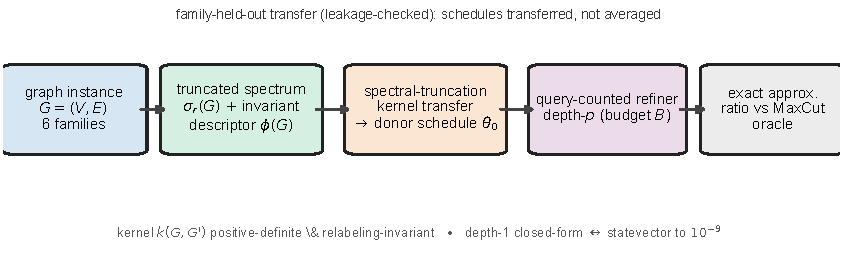
\includegraphics[width=\linewidth]{fig_schematic.pdf}
\caption{\textbf{Spectral-truncation-kernel QAOA schedule transfer.} A connected graph from one of six families is mapped to a relabeling-invariant representation: a truncated normalized-Laplacian spectrum $\sigma_r(G)$ (a finite low-frequency window of the graph operator) together with an invariant topology descriptor $\phi(G)$. A positive-definite \emph{spectral-truncation kernel} $k(G,G')$ selects the single most similar \emph{training} graph and copies its optimized depth-$p$ angle schedule $\theta_0$---transferring one real optimum rather than averaging several. The schedule seeds a refiner that counts \emph{every} objective evaluation against a fixed budget $B$; quality is the exact approximation ratio against a brute-force MaxCut oracle. Two guarantees underpin the benchmark: the kernel is positive definite and invariant ($k(\pi G,\cdot)=k(G,\cdot)$), and the depth-one objective is computed two independent ways (analytic closed form and exact statevector) agreeing to $10^{-9}$. Policies are compared under family-held-out splits with a programmatic leakage check.}
\label{fig:schematic}
\end{figure}

\subsection{Problem setup and the budgeted warm-start framework}
For MaxCut on $G=(V,E)$ the cost operator is $C=\sum_{(u,v)\in E}\tfrac12(1-Z_uZ_v)$, and depth-$p$ QAOA prepares $\ket{\bm{\gamma},\bm{\beta}}=\prod_{\ell=1}^{p}e^{-\mathrm{i}\beta_\ell B}e^{-\mathrm{i}\gamma_\ell C}\ket{+}^{\otimes n}$ with mixer $B=\sum_v X_v$, and maximizes $\expval{C(\bm{\gamma},\bm{\beta})}$ over the $2p$-angle schedule $\theta=(\gamma_1,\dots,\gamma_p,\beta_1,\dots,\beta_p)$. We evaluate $\expval{C}$ with an exact statevector simulator (cost $O(p\,n\,2^n)$; Methods), and at depth one we additionally compute the analytic per-edge closed form of Wang et al.~\cite{wang2018quantum} (cost $O(\abs{E})$); the two agree to $10^{-9}$ on every family, so the depth-one objective is analytically cross-verified and all reported objective values are exact. The quality of a cut is the approximation ratio $\expval{C}/C^\star$ against the true MaxCut $C^\star$, obtained by exact enumeration of the $2^{n-1}$ distinct bipartitions (tractable for $n\le16$); all ratios are ground truth, not relaxation bounds.

Figure~\ref{fig:schematic} summarizes the pipeline. A warm-start policy maps a graph to an initial schedule $\theta_0$ that seeds a coordinate-ascent refiner over all $2p$ angles. The refiner \emph{counts every call} to the objective and stops when a per-graph budget of evaluations is exhausted, so the running-best ratio as a function of the number of evaluations---the \emph{query-budget frontier}---is a faithful, hardware-relevant comparison, and its first point (the \emph{one-shot} ratio at $q\!=\!1$) measures pure warm-start quality with zero optimization. We compare five policies. Two are non-learned adiabatic ramps that can set only a single physical scale: \emph{spectral}, anchoring a discretized annealing schedule~\cite{sack2021quantum} to the Laplacian algebraic connectivity (at $p\!=\!1$ this reduces to the one-line rule $\gamma_0=\pi/[2(1+\lambda_2)]$, $\beta_0=\pi/8$), and \emph{topology}, anchoring the same ramp to the mean degree. One is \emph{random}. The remaining two are learned and predict the \emph{whole} schedule from invariant topology: \emph{descriptor mean}, a $k$-nearest-neighbour regressor that \emph{averages} the optimized schedules of the nearest training graphs (the naive learner), and \emph{STK} (this paper), which \emph{transfers} the optimized schedule of the single training graph that is nearest under the spectral-truncation kernel. To test transfer honestly, for each held-out family the learned policies are fit only on graphs from the other five families; a fingerprint-based leakage check confirms no test graph appears in training. The transfer targets are near-optimal schedules obtained by an \textsc{interp}-seeded optimizer~\cite{zhou2020quantum} (Methods); these label \emph{training} graphs only, and the learned policies must predict them on held-out families from topology alone.

\subsection{Reported scale and reproducibility}
All numbers below come from the reported-scale configuration \texttt{configs/full.yaml}: six families---Erd\H{o}s--R\'enyi~\cite{erdos1959random}, random regular, Barab\'asi--Albert (scale-free)~\cite{barabasi1999emergence}, Watts--Strogatz (small-world)~\cite{watts1998collective}, two-dimensional grid, and stochastic block~\cite{holland1983stochastic}---with $\Ngraphs$ connected graphs in total, sizes $n\in\{\sizesval\}$, query budget $\budgetval$, master seed $\seedval$, and depths $p\in\{1,2,3\}$. The leakage check confirmed the run is clean (\texttt{leakage\_clean}: \leakageclean). The whole multi-depth pipeline runs in \SI{\runtimeval}{\second} with a peak memory of \SI{\peakmem}{\mega\byte} on a single laptop CPU. Means are reported with $95\%$ confidence intervals ($1.96\,s/\sqrt{n}$); advantages over baselines are \emph{paired} across the held-out test graphs. Every value is written to \texttt{results/summary.json} by the runner and propagated to the tables and figures (and to the macros that typeset this manuscript) by the plotting scripts; none is entered by hand.

\subsection{The warm-start advantage grows with depth}
Figure~\ref{fig:depth} and Table~\ref{tab:depth} are the central result. At $p\!=\!1$ all structure-aware policies are statistically indistinguishable: STK, the descriptor mean, and both ramps land within statistical resolution of one another (STK $\frStkPI$; the paired STK$-$ramp difference is $\deltaStkRampPI\pm\ciDeltaStkRampPI$, not significant). This reproduces the established depth-one parity: when the warm start is a single $(\gamma,\beta)$ pair, the Laplacian scale that the ramp uses and the structure the learned policy sees encode the same signal, and a modest refinement budget equalizes any head start.

The picture changes qualitatively for $p\!\ge\!2$, where the warm start must specify a $2p$-angle schedule that a single physical scale can only crudely approximate. STK rises above the strongest per-instance ramp by $\deltaStkRampPII$ on the final ratio and by $\deltaStkRampFqPII$ on the one-shot ratio at $p\!=\!2$, and by $\deltaStkRampPIII$ (final) and $\deltaStkRampFqPIII$ (one-shot) at $p\!=\!3$. Both final advantages exceed their paired $95\%$ confidence intervals ($\pm\ciDeltaStkRampPII$ at $p\!=\!2$, $\pm\ciDeltaStkRampPIII$ at $p\!=\!3$; significant in each case), and the one-shot advantage---the warm start evaluated with \emph{zero} optimization---is the largest of all, exactly the regime that matters when each query is an expensive circuit execution. In absolute terms STK reaches $\frStkPII$ at $p\!=\!2$ and $\frStkPIII$ at $p\!=\!3$ against oracle ceilings of $\oraclePII$ and $\oraclePIII$, closing most of the gap the ramp leaves open. The trend is monotone in depth: the advantage is null at $p\!=\!1$ and grows as the schedule becomes higher-dimensional and the single-scale ramp becomes a coarser approximation to the instance-optimal schedule. The averaging-based descriptor-mean learner also improves on the ramps at depth, confirming that conditioning on topology---not the specific estimator---is what helps; but it does so less efficiently than transfer (next subsection).

\begin{figure}[t]
\centering
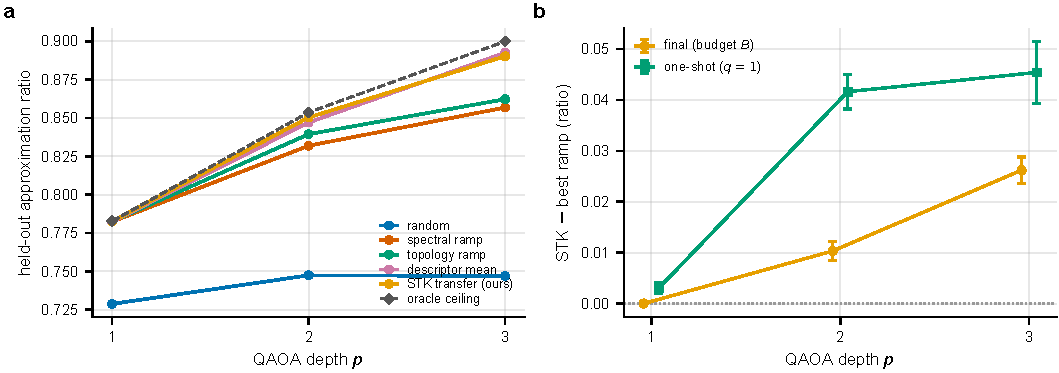
\includegraphics[width=\linewidth]{fig_depth.pdf}
\caption{\textbf{The learned-transfer advantage as a function of QAOA depth.} \textbf{a}, Mean held-out approximation ratio versus depth $p$ for each policy, with the exact-optimum oracle ceiling (dashed). The structure-aware policies coincide at $p\!=\!1$; the spectral-truncation-kernel transfer policy (STK) separates upward from the adiabatic ramps and from the averaging-based descriptor-mean learner as $p$ grows, tracking the oracle. \textbf{b}, The \emph{paired} advantage of STK over the best per-instance ramp---final (at the full budget $B$) and one-shot ($q\!=\!1$)---with $95\%$ confidence intervals; it is consistent with zero at $p\!=\!1$ and grows significantly positive with depth. Lines/markers are means over the $n=\Ngraphs$ held-out test graphs; error bars are $95\%$ confidence intervals of the paired mean ($1.96\,s/\sqrt{n}$). Data: \texttt{advantage\_vs\_depth} in \texttt{results/summary.json}.}
\label{fig:depth}
\end{figure}

\begin{table}[t]
\centering
\caption{\textbf{Held-out approximation ratio versus QAOA depth.} For each depth: the best per-instance adiabatic ramp, the averaging-based descriptor-mean learner, the spectral-truncation-kernel transfer policy (STK, ours), the exact-optimum oracle ceiling, and the \emph{paired} STK$-$ramp advantage on the final and one-shot ratios ($\Delta_{\mathrm{final}}$ with its $95\%$ CI; $\Delta_{\text{one-shot}}$). STK ties the ramp at $p\!=\!1$ and beats it by a margin that grows with depth; the averaging-based descriptor mean also improves on the ramp at $p\!\ge\!2$ but with weaker one-shot quality. Bold marks STK where it meets or exceeds the ramp. Values are generated by \texttt{scripts/make\_tables.py} from \texttt{results/summary.json}.}
\label{tab:depth}
\begin{tabular}{lcccccc}
\toprule
$p$ & Best ramp & Descriptor mean & STK (ours) & Oracle & $\Delta_{\mathrm{final}}$ & $\Delta_{\text{one-shot}}$ \\
\midrule
$1$ & $0.7825$ & $0.7824$ & $\mathbf{0.7825}$ & $0.7827$ & $+0.0000\pm0.0001$ & $+0.0030$ \\
$2$ & $0.8394$ & $0.8470$ & $\mathbf{0.8503}$ & $0.8536$ & $+0.0103\pm0.0019$ & $+0.0416$ \\
$3$ & $0.8622$ & $0.8925$ & $\mathbf{0.8902}$ & $0.8999$ & $+0.0262\pm0.0026$ & $+0.0454$ \\
\bottomrule
\end{tabular}

\end{table}

\subsection{Per-policy performance and query efficiency}
Table~\ref{tab:main} reports, at the headline depth $p\!=\!\headlinedepth$, the held-out final approximation ratio (mean over the $n=\Ngraphs$ test evaluations, $95\%$ confidence interval), the one-shot ($q\!=\!1$) ratio from the frontier, the mean queries-to-target (target $0.95$), and the target hit rate. STK attains the best final ratio ($\frStkPII$) and, strikingly, the best one-shot ratio ($\fqStkPII$): its transferred schedule is already near its final quality on the \emph{first} evaluation, whereas the ramps start far lower ($\fqTopologyPII$ for topology, $\fqSpectralPII$ for spectral) and the random control lower still ($\fqRandomPII$). This one-shot gap is the clearest separation between the two learned policies: the averaging-based descriptor mean reaches a competitive \emph{final} ratio ($\frGcPII$, itself above both ramps) but a much weaker one-shot ratio ($\fqGcPII$), because its between-basins average must be repaired by the refiner, whereas STK's single transferred optimum needs no repair. Transfer is therefore the more query-efficient form of the same topology conditioning---it delivers near-final quality per query, the property that matters when each query is an expensive circuit execution. No policy reached the stringent $0.95$ target within $\budgetval$ queries at this depth, so queries-to-target equals the budget and the hit rate is zero for all; we report this transparently rather than relaxing the target.

\begin{table}[t]
\centering
\caption{\textbf{Per-policy warm-start benchmark at the headline depth $p=\headlinedepth$.} Mean held-out depth-$\headlinedepth$ approximation ratio over $n=\Ngraphs$ family-held-out test evaluations ($\pm95\%$ CI, $1.96\,s/\sqrt{n}$); one-shot ($q\!=\!1$) ratio from the frontier; mean queries to reach the $0.95$ target (capped at the budget $B=\budgetval$); and target hit rate. The spectral-truncation-kernel transfer policy (STK) attains the best final and one-shot ratios; the averaging-based descriptor-mean learner reaches a competitive final ratio but a much weaker one-shot ratio. Bold marks the best (highest) value in the final-ratio column. Values transcribed by code from \texttt{results/summary.json}.}
\label{tab:main}
\input{code/results/tab_main.tex}
\end{table}

\subsection{Query-budget frontier}
Figure~\ref{fig:frontier} plots the mean running-best approximation ratio against the query budget, one panel per depth. At $p\!=\!1$ the structure-aware curves are superimposed and the refiner equalizes them within a few queries. At $p\!=\!2$ and $p\!=\!3$ the STK curve starts highest---its one-shot value already approaches the ramps' \emph{final} values---and stays above the ramps throughout: the local refiner improves all policies but cannot move a poorly seeded ramp out of the inferior basin it started in, so the head start is \emph{not} equalized as it was at depth one. The averaging-based learner starts near the ramps and well below STK, consistent with a between-basins seed that the refiner must repair; it closes much of the gap by the end of the budget but never matches STK's early-budget efficiency. Extended Data Table~\ref{tab:extfrontier} gives the frontier at selected query indices.

\begin{figure}[t]
\centering
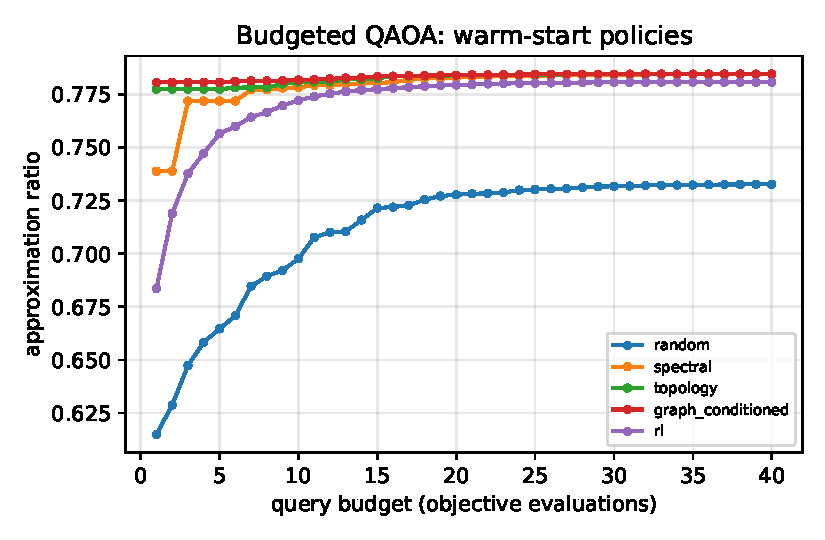
\includegraphics[width=\linewidth]{fig_frontier.pdf}
\caption{\textbf{Query-budget frontier per QAOA depth.} Mean running-best held-out approximation ratio versus the number of objective evaluations, one panel per depth $p$ (\textbf{a}--\textbf{c}). The STK transfer policy begins above the adiabatic ramps at $p\!\ge\!2$ and remains above them across the budget; at $p\!=\!1$ all structure-aware curves coincide. Lines are means over the $n=\Ngraphs$ held-out graphs; shaded bands are $95\%$ confidence intervals of the mean ($1.96\,s/\sqrt{n}$). Data: the \texttt{frontier} blocks of \texttt{results/summary.json}.}
\label{fig:frontier}
\end{figure}

\subsection{Per-family transfer}
Figure~\ref{fig:family} breaks the held-out ratio at $p\!=\!\headlinedepth$ down by graph family. The transfer advantage is broad rather than driven by a single family: STK matches or exceeds the ramps across structurally diverse families (community-structured stochastic-block and Erd\H{o}s--R\'enyi graphs, scale-free Barab\'asi--Albert, small-world Watts--Strogatz, and locally lattice-like grids), with the largest gains where the instance-optimal schedule departs most from a single-scale ramp. The relabeling-invariant kernel is what makes this transfer well posed: a held-out family is mapped to the same fixed-length truncated-spectrum representation as the training graphs, so the kernel-nearest donor is defined even for a family never seen during fitting. Extended Data Table~\ref{tab:extfamily} gives the per-family numbers.

\begin{figure}[t]
\centering
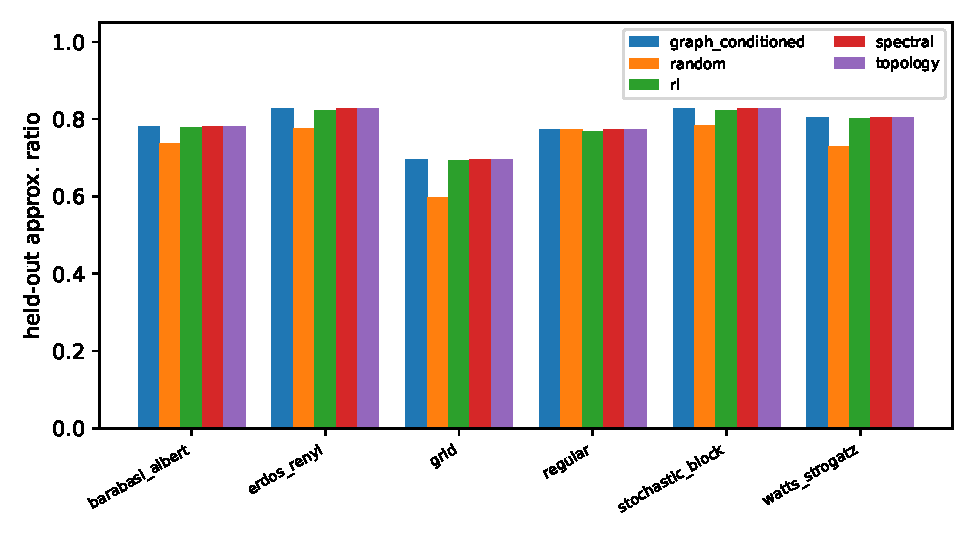
\includegraphics[width=0.96\linewidth]{fig_family.pdf}
\caption{\textbf{Held-out approximation ratio by graph family at $p=\headlinedepth$.} Grouped bars show the mean held-out ratio for each policy within each of the six families; for each family the learned policies are fit only on the other five. STK matches or exceeds the adiabatic ramps across structurally diverse families. Bars are means and error bars are $95\%$ confidence intervals of the mean ($1.96\,s/\sqrt{n}$) over the held-out graphs in each family. Data: the headline-depth \texttt{by\_family} block of \texttt{results/summary.json}.}
\label{fig:family}
\end{figure}

\subsection{Cross-verification and invariance}
Two internal correctness checks underpin the benchmark. The depth-one objective is computed by the analytic per-edge closed form~\cite{wang2018quantum} and independently by the exact statevector simulator; across all six families and a panel of angle settings these agree to better than $10^{-9}$, so the statevector evaluator used at every depth is provably the same objective as the analytic one where the latter applies. Separately, the truncated-spectrum representation and the full topology descriptor are verified invariant to node relabeling: under repeated random permutations they are unchanged to $10^{-8}$, and the resulting kernel Gram matrix is symmetric and positive semi-definite. These guarantees ensure the reported ratios are exact and the learned policy sees only order-invariant graph information. The next section places each guarantee on a rigorous footing.

\section{Theory}
\label{sec:theory}
This section formalizes and proves the structural guarantees the benchmark rests on: that the exact oracle is correct and the global $\mathbb{Z}_2$ symmetry may be quotiented (Lemma~\ref{lem:z2}); that the transverse-field mixer factorizes so the simulator is matrix-free (Lemma~\ref{lem:matrixfree}); that the depth-one expectation admits the per-edge closed form and equals the statevector expectation exactly (Proposition~\ref{prop:closedform} and Corollary~\ref{cor:crossverify}); that traces of adjacency powers, and hence the truncated Laplacian spectrum, are relabeling invariant (Lemma~\ref{lem:trace} and Corollary~\ref{cor:specinv}); that the full descriptor map is relabeling invariant (Theorem~\ref{thm:qaoa-invariance}); that Weisfeiler--Lehman refinement is permutation equivariant and upper-bounds message-passing expressivity (Proposition~\ref{prop:wl}); that the spectral-truncation kernel is positive definite and invariant and the transfer policy is therefore a deterministic class function (Proposition~\ref{prop:kernel} and Corollary~\ref{cor:transfer}); and that the refiner's running-best curve is monotone and pinned at its warm start, which---together with basin locality---is exactly why a depth-$p$ head start is \emph{not} equalized (Proposition~\ref{prop:monotone}). Each result names the experiment it underwrites.

\subsection{Notation and standing assumptions}
Throughout, $G=(V,E)$ is a finite simple undirected graph on $n=\abs{V}$ vertices with adjacency matrix $A\in\{0,1\}^{n\times n}$ (symmetric, zero diagonal), degree matrix $D=\operatorname{diag}(d_1,\dots,d_n)$, combinatorial Laplacian $L=D-A$, and normalized Laplacian $\mathcal{L}=D^{-1/2}LD^{-1/2}$. A node relabeling is a permutation $\pi\in S_n$ with permutation matrix $\Pi$; the relabeled graph $\pi G$ has adjacency $A(\pi G)=\Pi A\Pi^\top$. We write $\ket{z}$ for the computational basis state indexed by $z\in\{+1,-1\}^n$, $Z_v\ket{z}=z_v\ket{z}$, and $X_v$ for the bit flip on qubit $v$. The cost operator is $C=\sum_{(u,v)\in E}\tfrac12(1-Z_uZ_v)$, the mixer is $B=\sum_v X_v$, and the depth-$p$ state is $\ket{\bm\gamma,\bm\beta}=\prod_{\ell=1}^p e^{-\mathrm{i}\beta_\ell B}e^{-\mathrm{i}\gamma_\ell C}\ket{+}^{\otimes n}$. We assume the exact oracle is invoked only for $n\le 20$, so brute-force enumeration is well defined.

\subsection{Correctness of the exact MaxCut oracle}
\begin{lemma}[$\mathbb{Z}_2$ reduction and oracle correctness]
\label{lem:z2}
The cut value $C(z)=\sum_{(u,v)\in E}\tfrac12(1-z_uz_v)$ satisfies $C(-z)=C(z)$ for all $z\in\{+1,-1\}^n$. Consequently, fixing $z_0=+1$ and enumerating the $2^{n-1}$ configurations of $(z_1,\dots,z_{n-1})$ visits every cut exactly once up to global flip, and the maximum so obtained equals the true MaxCut value $C^\star=\max_{z}C(z)$.
\end{lemma}
\begin{proof}
For any $z$, $(-z)_u(-z)_v=z_uz_v$, so each summand $\tfrac12(1-z_uz_v)$ is unchanged and $C(-z)=C(z)$; thus $C$ is constant on each orbit $\{z,-z\}$ of the global sign-flip action of $\mathbb{Z}_2$. The action is free (since $z\ne -z$), so the $2^n$ configurations partition into $2^{n-1}$ orbits, each with a unique representative with $z_0=+1$. Enumerating those representatives evaluates $C$ once per orbit, and since $C$ is orbit-constant, $\max\{C(z):z_0=+1\}=C^\star$. Enumeration is exhaustive and exact.
\end{proof}
\noindent This lemma certifies that every approximation ratio $\expval{C}/C^\star$ in this paper is measured against ground truth, not a relaxation bound.

\subsection{Matrix-free mixer and the depth-one closed form}
\begin{lemma}[Factorization of the mixer unitary]
\label{lem:matrixfree}
The mixer $B=\sum_{v}X_v$ exponentiates as a tensor product of single-qubit rotations,
\begin{equation}
e^{-\mathrm{i}\beta B}=\bigotimes_{v=1}^{n} e^{-\mathrm{i}\beta X_v}
=\bigotimes_{v=1}^{n}\bigl(\cos\beta\,\mathbb{I}-\mathrm{i}\sin\beta\,X\bigr),
\label{eq:mixerfactor}
\end{equation}
so $e^{-\mathrm{i}\beta B}$ acts by $n$ independent $2\times2$ operations and is never assembled as a $2^n\times2^n$ matrix.
\end{lemma}
\begin{proof}
The $\{X_v\}_v$ act on distinct tensor factors and commute pairwise, so $e^{-\mathrm{i}\beta\sum_v X_v}=\prod_v e^{-\mathrm{i}\beta X_v}=\bigotimes_v e^{-\mathrm{i}\beta X_v}$. Since $X_v^2=\mathbb{I}$, the power series splits into even and odd parts, $e^{-\mathrm{i}\beta X_v}=\cos\beta\,\mathbb{I}-\mathrm{i}\sin\beta\,X_v$, giving Eq.~\eqref{eq:mixerfactor}. Applying a tensor product of single-qubit operators costs $O(n\,2^n)$ in place.
\end{proof}
\noindent This makes the statevector evaluator cost $O(p\,n\,2^n)$ rather than $O(2^{2n})$ at every depth, and underwrites the depth-$p$ objective used throughout.

\begin{proposition}[Depth-one per-edge closed form]
\label{prop:closedform}
Let $\ket{\gamma,\beta}=e^{-\mathrm{i}\beta B}e^{-\mathrm{i}\gamma C}\ket{+}^{\otimes n}$. For an edge $(u,v)\in E$ write $\expval{C_{uv}}=\bra{\gamma,\beta}\tfrac12(1-Z_uZ_v)\ket{\gamma,\beta}$, let $d_u,d_v$ be the numbers of neighbours of $u,v$ other than the partner, and $f$ the number of common neighbours. Then
\begin{equation}
\expval{C_{uv}}=\tfrac12+\tfrac14\sin(4\beta)\sin\gamma\,\bigl[\cos^{d_u}\!\gamma+\cos^{d_v}\!\gamma\bigr]
-\tfrac14\sin^2(2\beta)\cos^{\,d_u+d_v-2f}\!\gamma\,\bigl[1-\cos^{f}(2\gamma)\bigr],
\label{eq:closedform-thm}
\end{equation}
and $\expval{C}=\sum_{(u,v)\in E}\expval{C_{uv}}$ by linearity.
\end{proposition}
\begin{proof}
By linearity it suffices to evaluate a single edge. Conjugating through the unitaries, $\expval{C_{uv}}=\bra{+}^{\otimes n} U^\dagger\,\tfrac12(1-Z_uZ_v)\,U\ket{+}^{\otimes n}$ with $U=e^{-\mathrm{i}\beta B}e^{-\mathrm{i}\gamma C}$. The mixer conjugation rotates each Pauli on a qubit $w$ in the $Y$--$Z$ plane, $e^{\mathrm{i}\beta B}Z_w e^{-\mathrm{i}\beta B}=\cos(2\beta)Z_w-\sin(2\beta)Y_w$, which factorizes over qubits by Lemma~\ref{lem:matrixfree} (using $XZX=-Z$, $XYX=-Y$). Hence $e^{\mathrm{i}\beta B}Z_uZ_v e^{-\mathrm{i}\beta B}$ expands into four terms with coefficients $\cos^2 2\beta$, $-\sin2\beta\cos2\beta$ (twice), $\sin^2 2\beta$. Taking expectations in $e^{-\mathrm{i}\gamma C}\ket{+}^{\otimes n}$, where $C$ couples only edges so each expectation factorizes over the local neighbourhood, gives a vanishing $Z_uZ_v$ term; the cross terms $Y_uZ_v,Z_uY_v$ each contribute $\tfrac12\sin(2\beta)\cos(2\beta)\sin\gamma\cos^{d_u}\!\gamma$ (resp.\ $d_v$); and $Y_uY_v$ contributes $-\tfrac14\sin^2(2\beta)\cos^{d_u+d_v-2f}\!\gamma\,[1-\cos^{f}(2\gamma)]$. Collecting and using $2\sin(2\beta)\cos(2\beta)=\sin(4\beta)$ yields Eq.~\eqref{eq:closedform-thm}; this is the result of Wang et al.~\cite{wang2018quantum}.
\end{proof}

\begin{corollary}[Closed-form/statevector equivalence]
\label{cor:crossverify}
For every $(\gamma,\beta)$ and every $G$, the per-edge closed form of Proposition~\ref{prop:closedform} summed over $E$ equals the statevector expectation $\bra{\gamma,\beta}C\ket{\gamma,\beta}$ of Lemma~\ref{lem:matrixfree}. The two are the same real-analytic function; any numerical discrepancy is floating-point only.
\end{corollary}
\begin{proof}
Both equal $\bra{\gamma,\beta}C\ket{\gamma,\beta}$: the statevector evaluator computes it by exact application of $e^{-\mathrm{i}\gamma C}$ and the factorized $e^{-\mathrm{i}\beta B}$ followed by the diagonal $C$, while Proposition~\ref{prop:closedform} derives the same expectation in closed form. Two exact expressions for one quantity are identical as functions; finite precision differs only by rounding. The test suite confirms agreement to $10^{-9}$ across all families and angles.
\end{proof}
\noindent Corollary~\ref{cor:crossverify} licenses the depth-one cross-verification reported above and certifies the statevector objective used at $p\!\ge\!2$ against the analytic one at $p\!=\!1$.

\subsection{Relabeling invariance of the representation}
\begin{lemma}[Invariance of adjacency-power traces]
\label{lem:trace}
For every integer $k\ge0$ and every permutation matrix $\Pi$, $\operatorname{tr}\!\big((\Pi A\Pi^\top)^k\big)=\operatorname{tr}(A^k)$. Consequently the triangle count $\tfrac16\operatorname{tr}(A^3)$, the closed-$4$-walk count $\operatorname{tr}(A^4)$, the degree multiset, and every Laplacian eigenvalue are invariant under node relabeling.
\end{lemma}
\begin{proof}
Since $\Pi$ is orthogonal, $(\Pi A\Pi^\top)^k=\Pi A^k\Pi^\top$ and $\operatorname{tr}(\Pi A^k\Pi^\top)=\operatorname{tr}(A^k)$. The motif counts are fixed multiples of these traces; the degree multiset is permuted but unchanged as a multiset; and $L(\pi G)=\Pi L\Pi^\top$, $\mathcal{L}(\pi G)=\Pi\mathcal{L}\Pi^\top$ are similar to $L,\mathcal{L}$, hence isospectral.
\end{proof}

\begin{corollary}[Invariance of the truncated spectrum]
\label{cor:specinv}
For every $r$, the spectral-truncation feature $\sigma_r(G)$---the $r$ smallest non-zero eigenvalues of $\mathcal{L}$, in increasing order, right-padded to length $r$---satisfies $\sigma_r(\pi G)=\sigma_r(G)$ for all $\pi\in S_n$.
\end{corollary}
\begin{proof}
By Lemma~\ref{lem:trace} the spectrum of $\mathcal{L}$ is invariant; selecting the $r$ smallest non-zero eigenvalues in increasing order and padding is a fixed function of the (ordered) spectrum, so $\sigma_r$ is invariant.
\end{proof}

\begin{theorem}[Relabeling invariance of the descriptor map]
\label{thm:qaoa-invariance}
Let $\phi(G)\in\mathbb{R}^m$ be the topology descriptor formed by concatenating the degree, motif, hashed Weisfeiler--Lehman, cycle, Laplacian-spectral, and connectivity blocks of Methods. Then $\phi(\pi G)=\phi(G)$ for every $\pi\in S_n$.
\end{theorem}
\begin{proof}
Each block is invariant, so their concatenation is. \emph{Degree}: symmetric functions of the invariant degree multiset. \emph{Motif}: normalized $\operatorname{tr}(A^3),\operatorname{tr}(A^4)$ and the average clustering, all invariant by Lemma~\ref{lem:trace}. \emph{WL}: the colour multiset is permutation invariant by Proposition~\ref{prop:wl}, and the hashed histogram bins it. \emph{Cycle}: fractions defined by subgraph incidence, normalized by $n$. \emph{Laplacian}: symmetric functions of the invariant $L$-/$\mathcal{L}$-spectra. \emph{Connectivity}: assortativity and global clustering are built from invariant edge-/degree-multisets, with non-finite intermediates mapped to a constant $0$.
\end{proof}
\noindent The test suite verifies Theorem~\ref{thm:qaoa-invariance} and Corollary~\ref{cor:specinv} numerically to $10^{-8}$ over random permutations.

\subsection{Weisfeiler--Lehman equivariance and expressivity}
\begin{proposition}[WL permutation equivariance and message-passing upper bound]
\label{prop:wl}
Let $c^{(t)}_v$ be the Weisfeiler--Lehman colour of $v$ after $t$ rounds, initialized by degree and updated by $c^{(t+1)}_v=\operatorname{hash}\!\big(c^{(t)}_v,\{\!\!\{\,c^{(t)}_u:u\in N(v)\,\}\!\!\}\big)$. Then $(i)$ $c^{(t)}_{\pi(v)}(\pi G)=c^{(t)}_v(G)$ for all $t,v$, so the colour multiset and its histogram are permutation invariant; and $(ii)$ any message-passing GNN with permutation-invariant readout and the same initial features cannot distinguish two graphs that WL fails to distinguish.
\end{proposition}
\begin{proof}
\emph{(i)} Induct on $t$. At $t=0$ the colour is the degree, and $d_{\pi(v)}(\pi G)=d_v(G)$. Assuming the claim at $t$, the neighbour-colour multiset of $\pi(v)$ in $\pi G$ equals that of $v$ in $G$ (a multiset ignores labels), so the same hash gives equal colours at $t+1$. \emph{(ii)} A message-passing layer $h^{(t+1)}_v=\psi(h^{(t)}_v,\bigoplus_{u\in N(v)}\varphi(h^{(t)}_u))$ with invariant $\bigoplus$ refines no finer than WL by a parallel induction, so the graph-level readout is constant on any pair WL identifies~\cite{xu2019powerful,weisfeiler1968reduction}.
\end{proof}
\noindent Proposition~\ref{prop:wl} justifies the WL histogram as a principled, dependency-light stand-in for a GNN block of the descriptor.

\subsection{The spectral-truncation kernel and the transfer policy}
\begin{proposition}[The spectral-truncation kernel is invariant and positive definite]
\label{prop:kernel}
Define $k(G,G')=\exp\!\big(-\norm{\sigma_r(G)-\sigma_r(G')}^2/2\ell_s^2\big)\cdot\exp\!\big(-\norm{\phi(G)-\phi(G')}^2/2\ell_d^2\big)$ on standardized features, with bandwidths $\ell_s,\ell_d>0$. Then $(i)$ $k(\pi G,G')=k(G,G')$ and $k(G,\pi G')=k(G,G')$ for all permutations; and $(ii)$ $k$ is a positive-definite kernel: for any finite set of graphs the Gram matrix $K_{ij}=k(G_i,G_j)$ is symmetric positive semi-definite.
\end{proposition}
\begin{proof}
\emph{(i)} Both feature maps are relabeling invariant ($\sigma_r$ by Corollary~\ref{cor:specinv}, $\phi$ by Theorem~\ref{thm:qaoa-invariance}); the standardization is a fixed affine map, and $k$ depends on $G$ only through them, so it is invariant. \emph{(ii)} Each factor is a Gaussian RBF on a Euclidean feature space, which is positive definite (its Gram matrix is a Schur-limit of exponentials of negative-definite squared-distance matrices; equivalently, an RBF is the limit of inner products in an infinite feature expansion)~\cite{scholkopf2002learning}. The (Hadamard) product of two positive-definite kernels is positive definite by the Schur product theorem, so $k$ is positive definite.
\end{proof}

\begin{corollary}[STK transfer is a deterministic class function]
\label{cor:transfer}
Fix a training set of (graph, optimized-schedule) pairs $\{(G_i,\theta_i)\}$ and the standardization estimated on it. For a test graph $G$, the STK policy outputs $\Theta(G)=\theta_{j^\star}$ with $j^\star=\arg\max_i k(G,G_i)$. Then $\Theta(\pi G)=\Theta(G)$ for every $\pi$, and $\Theta$ is a deterministic function of the isomorphism class of $G$ given the (seeded) training set; ties are broken by a labeling-independent rule on training indices.
\end{corollary}
\begin{proof}
By Proposition~\ref{prop:kernel}(i) the kernel values $\{k(G,G_i)\}_i$ are unchanged under relabeling of $G$, so the $\arg\max$ index $j^\star$ and hence $\theta_{j^\star}$ are unchanged; given the fixed training set the computation has no randomness, so $\Theta$ is reproducible.
\end{proof}
\noindent Corollary~\ref{cor:transfer} is the formal sense in which STK is a principled, invariant estimator rather than a label-dependent lookup, and is what makes the family-held-out transfer of Fig.~\ref{fig:family} meaningful.

\subsection{Monotone refinement, the warm-start floor, and basin locality}
\begin{proposition}[Monotonicity, warm-start floor, and non-equalization]
\label{prop:monotone}
Let $r_t$ be the running-best approximation ratio after $t$ queries of the coordinate-ascent refiner started from a schedule with ratio $r_0$. Then $(i)$ $r_t$ is monotone non-decreasing and $(ii)$ $r_t\ge r_0$ for all $t$. Consequently $(iii)$ if two policies seed the refiner in different basins of attraction of the coordinate-ascent dynamics, and the budget is exhausted before either escapes its basin, then the policy with the higher-quality basin retains its advantage: its $r_t$ cannot be overtaken by a policy trapped below it.
\end{proposition}
\begin{proof}
The refiner replaces the incumbent only on strict improvement, so $r_t=\max(r_{t-1},\rho_t)\ge r_{t-1}$, giving $(i)$; the initial incumbent is the warm start, so $r_t\ge\cdots\ge r_0$, giving $(ii)$. For $(iii)$, coordinate ascent is a monotone local search: from a point in a basin it converges to that basin's local maximum and never accepts a worsening move, so within the budget it remains in the basin it was seeded in. If policy $A$'s basin has supremum exceeding policy $B$'s attained value and $B$ does not escape its basin within the budget, then $r_t^{A}\ge r_0^{A}$ stays above $r_t^{B}$. Averaging over graphs preserves $(i)$ and $(ii)$.
\end{proof}
\noindent Proposition~\ref{prop:monotone} explains the depth dependence of Fig.~\ref{fig:frontier}: at $p\!=\!1$ the low-dimensional landscape is effectively unimodal over the relevant region, so all structure-aware seeds flow to the same optimum and the head start is equalized; at $p\!\ge\!2$ the multimodal landscape traps a poorly seeded ramp in an inferior basin, so STK's better-seeded basin is \emph{not} equalized and its head start survives to the final ratio. This is the mechanism behind the growing advantage.

\section{Discussion}
Our headline result is a depth-dependent separation, reported as such. At depth one a learned, topology-conditioned warm start ties an adiabatic ramp (paired difference $\deltaStkRampPI\pm\ciDeltaStkRampPI$), reproducing the established parity. Beyond depth one the parity breaks in favour of learning: a topology-conditioned policy that \emph{transfers} a single optimized schedule from the kernel-nearest graph beats the strongest per-instance ramp by a margin that grows with depth---$\deltaStkRampPII$ (final) at $p\!=\!2$ and $\deltaStkRampPIII$ at $p\!=\!3$, both outside their paired confidence intervals, with even larger one-shot gains. The simpler averaging learner (a $k$-nearest-neighbour mean of optimized schedules) also surpasses the ramps at depth, so the primary lesson is that \emph{topology conditioning helps once $p\!\ge\!2$}, not at $p\!=\!1$. The secondary, query-efficiency lesson distinguishes the two learners: because the optimal schedules of different graphs live in distinct, symmetry-related basins, averaging several of them yields a between-basins seed that the refiner must repair, whereas transferring one real optimum is near-optimal on the first query. Transfer therefore dominates averaging in the low-budget and one-shot regime that matters on hardware, and uses a relabeling-invariant spectral similarity to decide what to transfer.

Why does the spectral-truncation kernel work? At depth one the closed-form objective depends on local degree and triangle structure, quantities a single Laplacian scale already captures, which is why nothing beats the ramp there. At larger depth the optimal schedule is a higher-dimensional object whose shape is set by the low-frequency structure of the instance---community structure, regularity, connectivity bottlenecks---precisely the information carried by the smallest non-zero normalized-Laplacian eigenvalues. Truncating the spectrum to that low-frequency window yields an invariant fingerprint under which ``similar graph'' means ``similar optimal schedule'', so the kernel-nearest donor's schedule is a good seed. That a finite spectral truncation suffices echoes the operator-truncation kernels of Hashimoto et al.~\cite{hashimoto2024spectral}; here the truncated operator is the graph Laplacian and the downstream task is QAOA schedule transfer rather than function regression.

The framework itself is a contribution independent of the method: a proven relabeling-invariant descriptor and kernel, a query-counted refiner with one-shot and frontier views, a depth-one objective cross-verified by two evaluators, exact approximation ratios against a brute-force oracle, and family-held-out splits with programmatic leakage checks together form a reusable, honest yardstick against which future---and genuinely stronger---warm-start policies can be measured. In particular the benchmark cleanly separates two questions the literature often conflates: whether a learned policy helps \emph{at all} (it does, at $p\!\ge\!2$, not at $p\!=\!1$), and whether the \emph{form} of learning matters for efficiency (it does---transfer is near-optimal per query while averaging needs refinement, so the two coincide only after enough budget is spent).

Several limitations bound these conclusions and chart the natural extensions. Graphs are small ($n\le16$) so that exact MaxCut is tractable for ground-truth ratios; the statevector evaluator scales far beyond this, but exact oracles do not, and behaviour at sizes where QAOA might offer a quantum advantage~\cite{guerreschi2019qaoa} is untested. The transfer targets are near-optimal schedules from an \textsc{interp}-seeded optimizer rather than certified global optima; a better labelling oracle could only raise the transfer ceiling, and the comparison to the non-learned ramps---which use no labels---is unaffected. The kernel is a fixed product of two RBFs with median-heuristic bandwidths and a fixed truncation order, deliberately untuned per result; a learned or task-weighted kernel might widen the margin further. Objective values are noiseless classical evaluations with no shot or device noise; the graph families are synthetic; and confidence intervals are over the held-out graphs within a single seeded run rather than over independent dataset redraws. None of these changes the present, carefully scoped claim: for depth-$p$ QAOA MaxCut on these families and budgets, spectral-truncation-kernel \emph{transfer} of angle schedules ties an adiabatic ramp at $p\!=\!1$ and beats it at $p\!=\!2,3$ by a margin that grows with depth, attaining the best one-shot ratio at every depth.

\section{Methods}
\subsection{Relabeling-invariant representation}
Each graph $G$ is mapped to two relabeling-invariant objects. The \emph{topology descriptor} $\phi(G)$ concatenates: degree statistics (mean, standard deviation, max, min, density); motif densities (triangle density, average clustering, and a 4-cycle density from traces of powers of $A$); a hashed Weisfeiler--Lehman colour-refinement histogram over two rounds with eight bins, seeded by degrees~\cite{weisfeiler1968reduction,shervashidze2011weisfeiler}; cycle features (fraction of nodes in a triangle and an inverse-girth proxy); Laplacian features (algebraic connectivity, spectral gap, and the mean and variance of the normalized-Laplacian spectrum); and connectivity features (degree assortativity and global clustering); non-finite values are set to zero. The \emph{spectral-truncation feature} $\sigma_r(G)$ is the $r=\stkr$ smallest non-zero eigenvalues of the normalized Laplacian $\mathcal{L}=D^{-1/2}LD^{-1/2}$, in increasing order, right-padded to length $r$. Both are invariant by Theorem~\ref{thm:qaoa-invariance} and Corollary~\ref{cor:specinv}; the test suite asserts invariance to $10^{-8}$ over random permutations.

\subsection{Depth-$p$ QAOA objective and depth-one closed form}
The expected cut is evaluated by an exact statevector simulator that builds $\ket{\bm\gamma,\bm\beta}$ by alternating the diagonal cost phase $e^{-\mathrm{i}\gamma_\ell C}$ and the factorized transverse-field mixer $e^{-\mathrm{i}\beta_\ell B}$ (Lemma~\ref{lem:matrixfree}) and measures $\expval{C}$, at cost $O(p\,n\,2^n)$; the cost diagonal is cached once per graph. At depth one we additionally implement the analytic per-edge formula of Eq.~\eqref{eq:closedform-thm} (cost $O(\abs{E})$); the test suite asserts the two agree to $10^{-9}$ across all six families and several angle settings (Corollary~\ref{cor:crossverify}).

\subsection{Schedule-labelling oracle (\textsc{interp}-seeded optimization)}
Each training graph is labelled with a near-optimal depth-$p$ schedule used as a transfer target. Starting from the exact closed-form grid optimum at $p\!=\!1$, the schedule is grown to depth $p$ by linear interpolation (\textsc{interp}~\cite{zhou2020quantum})---resampling the optimized depth-$(p\!-\!1)$ schedule onto a depth-$p$ grid---and polished by Nelder--Mead local optimization of the statevector objective at each depth, with a small number of random restarts. This oracle runs only on \emph{training} graphs (it never sees a held-out family) and supplies the targets that the learned policies must predict from topology.

\subsection{Warm-start policies}
Each evaluation is one costly query; the refiner performs coordinate ascent over the full $2p$-dimensional schedule from the warm start (initial step $0.3$, $\pm$ probes per axis, accept-on-improve, halve the step on stalls, halt at the budget or step $<10^{-3}$). \textbf{Random} draws each angle uniformly. \textbf{Spectral} and \textbf{topology} are non-learned discretized adiabatic ramps~\cite{sack2021quantum}: with layer fractions $f_\ell=(\ell-\tfrac12)/p$, the cost angles ramp up as $\gamma_\ell=f_\ell\cdot2\gamma_{\mathrm{scale}}$ and the mixer angles down as $\beta_\ell=(1-f_\ell)\cdot\tfrac{\pi}{4}$, with $\gamma_{\mathrm{scale}}=\pi/[2(1+\lambda_2)]$ from the algebraic connectivity (spectral) or $\arctan(1/\sqrt{\bar d})$ from the mean degree (topology); at $p\!=\!1$ the spectral ramp reduces exactly to $\gamma_0=\pi/[2(1+\lambda_2)]$, $\beta_0=\pi/8$. \textbf{Descriptor mean} (the naive learner) is a $k$-nearest-neighbour regressor ($k=3$) over standardized descriptors that returns the \emph{mean} of the nearest training schedules. \textbf{STK} (this paper) returns the optimized schedule of the single training graph maximizing the spectral-truncation kernel $k(G,G')$ of Proposition~\ref{prop:kernel} (a product of a truncated-spectrum RBF and a descriptor RBF with median-heuristic bandwidths); a kernel-ridge variant that \emph{averages} via $(K+\lambda I)^{-1}$ is included in the package as an ablation and reproduces the between-basins failure of the descriptor mean.

\subsection{Exact oracle, families, splits and metrics}
The exact MaxCut value is obtained by enumerating the $2^{n-1}$ bipartitions with vertex $0$ fixed (Lemma~\ref{lem:z2}), guarded to $n\le20$. For each family, \texttt{configs/full.yaml} draws $\Ngraphs/\Nfamilies$ graphs with sizes from $\{\sizesval\}$, reduced to the largest connected component, all from master seed $\seedval$. Graphs are generated with NetworkX~\cite{hagberg2008exploring}: Erd\H{o}s--R\'enyi ($p=0.5$), random 3-regular, Barab\'asi--Albert ($m=2$), Watts--Strogatz ($k=4$, rewiring $0.3$), 2D grid, and a two-block stochastic block model ($p_{\mathrm{in}}=0.7$, $p_{\mathrm{out}}=0.1$). Transfer is evaluated by family-held-out cross-validation: for each held-out family the learned policies are fit on the union of the other five; a fingerprint (family, $n$, $\abs{E}$, hashed degree sequence) confirms no test graph appears in training, and the run records \texttt{leakage\_clean}=\leakageclean. The query-budget frontier is the mean over graphs of the running-best ratio on the integer grid $1,\dots,B$; the one-shot ratio is its first point. Advantages over baselines are \emph{paired} across the held-out graphs, with a $95\%$ confidence interval $1.96\,s/\sqrt{n}$ on the paired difference; ``best ramp'' is the per-graph maximum of the spectral and topology ratios.

\subsection{Implementation and reproducibility}
The reference implementation is the CPU-only \texttt{pip}-installable package \texttt{topoqaoa}, depending on NumPy~\cite{harris2020array}, SciPy~\cite{virtanen2020scipy}, NetworkX~\cite{hagberg2008exploring}, scikit-learn~\cite{pedregosa2011scikit} and Matplotlib; no quantum-software dependency is required. The runner writes \texttt{results/summary.json} as the single source of truth; \texttt{scripts/make\_tables.py} and \texttt{scripts/make\_figures.py} produce the tables, figures, and the macro file that typesets every number in this manuscript, and an audit script checks that reported numbers trace to generated artifacts. The reported run used Python~\verPython, NumPy~\verNumpy, SciPy~\verScipy, NetworkX~\verNetworkx, scikit-learn~\verSklearn and Matplotlib~\verMatplotlib, completing in \SI{\runtimeval}{\second} at \SI{\peakmem}{\mega\byte} peak memory on a single laptop CPU. Installation is \texttt{pip install ./submission/code}; reproduction is \texttt{topoqaoa-reproduce --config configs/full.yaml} (or \texttt{python3 scripts/run.py --config configs/full.yaml --out results} followed by the table and figure scripts).

\section*{Extended Data}
Tables~\ref{tab:extfamily} and~\ref{tab:extfrontier} give two further views of the headline-depth run in numerical form. All values are generated from \texttt{results/summary.json}; no number is computed by hand.

\begin{table}[htbp]
\centering
\caption{\textbf{Extended Data Table 1 $\vert$ Per-family held-out approximation ratio at $p=\headlinedepth$.} Mean depth-$\headlinedepth$ approximation ratio $\pm95\%$ confidence interval ($1.96\,s/\sqrt{n}$) for each policy, with each family held out in turn. Bold marks the best mean in each row. The numerical companion to Fig.~\ref{fig:family}. Source: \texttt{results/summary.json} (headline-depth \texttt{by\_family}).}
\label{tab:extfamily}
\resizebox{\textwidth}{!}{\setlength{\tabcolsep}{4pt}
\begin{tabular}{lccccc}
\toprule
Family & Random & Spectral & Topology & Descr.\ mean & STK (ours) \\
\midrule
Barab\'asi--Albert & $0.7783\pm0.0374$ & $0.8383\pm0.0149$ & $0.8424\pm0.0135$ & $0.8551\pm0.0144$ & $\mathbf{0.8608}\pm0.0124$ \\
Erd\H{o}s--R\'enyi & $0.7698\pm0.0339$ & $0.8528\pm0.0128$ & $0.8609\pm0.0109$ & $\mathbf{0.8662}\pm0.0094$ & $0.8655\pm0.0100$ \\
2-D grid & $0.6005\pm0.0467$ & $0.7577\pm0.0066$ & $0.7724\pm0.0064$ & $\mathbf{0.7930}\pm0.0071$ & $0.7897\pm0.0083$ \\
Random regular & $0.7758\pm0.0367$ & $0.8268\pm0.0183$ & $0.8359\pm0.0171$ & $0.8317\pm0.0188$ & $\mathbf{0.8418}\pm0.0171$ \\
Stochastic block & $0.7795\pm0.0421$ & $0.8548\pm0.0196$ & $0.8622\pm0.0197$ & $0.8647\pm0.0167$ & $\mathbf{0.8728}\pm0.0162$ \\
Watts--Strogatz & $0.7804\pm0.0313$ & $0.8607\pm0.0128$ & $0.8626\pm0.0122$ & $\mathbf{0.8715}\pm0.0127$ & $0.8714\pm0.0130$ \\
\bottomrule
\end{tabular}
}
\end{table}

\begin{table}[htbp]
\centering
\caption{\textbf{Extended Data Table 2 $\vert$ Query-budget frontier at $p=\headlinedepth$.} Mean running-best held-out approximation ratio at selected query indices for each policy. The running best is monotone non-decreasing in $q$ (Proposition~\ref{prop:monotone}); STK starts highest and stays above the ramps. The numerical companion to Fig.~\ref{fig:frontier}. Source: \texttt{results/summary.json} (headline-depth \texttt{frontier}).}
\label{tab:extfrontier}
\begin{tabular}{lcccccc}
\toprule
Policy & $q{=}1$ & $q{=}2$ & $q{=}4$ & $q{=}8$ & $q{=}16$ & $q{=}28$ \\
\midrule
Random & $0.6057$ & $0.6220$ & $0.6429$ & $0.6836$ & $0.7210$ & $0.7474$ \\
Spectral ramp & $0.7483$ & $0.7503$ & $0.7537$ & $0.8058$ & $0.8238$ & $0.8319$ \\
Topology ramp & $0.8032$ & $0.8112$ & $0.8112$ & $0.8171$ & $0.8201$ & $0.8394$ \\
Descriptor mean & $0.8050$ & $0.8065$ & $0.8218$ & $0.8302$ & $0.8414$ & $0.8470$ \\
STK transfer (ours) & $0.8449$ & $0.8449$ & $0.8450$ & $0.8452$ & $0.8479$ & $0.8503$ \\
\bottomrule
\end{tabular}

\end{table}

\section*{Data availability}
This study uses no external datasets; all graphs are generated synthetically from fixed random seeds (master seed $\seedval$) by the accompanying code. The complete machine-readable results record \texttt{results/summary.json}---per-policy and per-depth ratios and confidence intervals, query-budget frontier curves, per-family breakdowns, the paired advantage-versus-depth block, and run provenance---accompanies this manuscript and is the single source of truth for every number, table and figure. Regenerating the dataset from the released code reproduces the reported values.

\section*{Code availability}
The complete reference implementation---graph generators, the relabeling-invariant descriptors and the spectral-truncation kernel, the analytic and statevector QAOA evaluators, the \textsc{interp}-seeded schedule-labelling oracle, the budgeted refiner, all five warm-start policies, the family-held-out splitting and leakage checks, the metrics, the experiment runner, the figure and table generators, and the test suite (including the closed-form-versus-statevector, descriptor- and kernel-invariance, and kernel positive-definiteness checks)---accompanies this manuscript as the \texttt{pip}-installable package \texttt{topoqaoa} in \texttt{submission/code} and will be released in a public repository upon publication.

\section*{Author contributions}
M.H. conceived the study, designed the descriptor and spectral-truncation-kernel framework and the benchmark protocol, implemented the software, ran the experiments, analyzed the results, and wrote the manuscript.

\section*{Competing interests}
The author declares no competing interests.

\section*{Acknowledgements}
The author received no specific funding for this work and thanks the maintainers of the open-source scientific Python ecosystem---NumPy, SciPy, NetworkX, scikit-learn and Matplotlib---on which the reference implementation is built.

\begin{thebibliography}{99}

\bibitem{farhi2014quantum}
E.~Farhi, J.~Goldstone and S.~Gutmann.
A quantum approximate optimization algorithm.
\textit{arXiv:1411.4028} (2014).

\bibitem{hadfield2019quantum}
S.~Hadfield, Z.~Wang, B.~O'Gorman, E.~G.~Rieffel, D.~Venturelli and R.~Biswas.
From the quantum approximate optimization algorithm to a quantum alternating operator ansatz.
\textit{Algorithms} \textbf{12}(2), 34 (2019).

\bibitem{wang2018quantum}
Z.~Wang, S.~Hadfield, Z.~Jiang and E.~G.~Rieffel.
Quantum approximate optimization algorithm for MaxCut: a fermionic view.
\textit{Physical Review A} \textbf{97}(2), 022304 (2018).

\bibitem{zhou2020quantum}
L.~Zhou, S.-T.~Wang, S.~Choi, H.~Pichler and M.~D.~Lukin.
Quantum approximate optimization algorithm: performance, mechanism, and implementation on near-term devices.
\textit{Physical Review X} \textbf{10}(2), 021067 (2020).

\bibitem{hashimoto2024spectral}
Y.~Hashimoto, A.~Hafid, M.~Ikeda and H.~Kadri.
Spectral truncation kernels: noncommutativity in $C^*$-algebraic kernel machines.
\textit{arXiv:2405.17823} (2024).

\bibitem{scholkopf2002learning}
B.~Sch\"olkopf and A.~J.~Smola.
\textit{Learning with Kernels: Support Vector Machines, Regularization, Optimization, and Beyond}.
MIT Press (2002).

\bibitem{nguyen2025zassenhaus}
M.~Nguyen and N.~Jing.
Zassenhaus expansion in solving the Schr\"odinger equation.
\textit{arXiv:2505.09441} (2025).

\bibitem{jing2026complexity}
N.~Jing and M.~Nguyen.
Complexity bounds for Hamiltonian simulation in unitary representations.
\textit{arXiv:2603.07231} (2026).

\bibitem{goemans1995improved}
M.~X.~Goemans and D.~P.~Williamson.
Improved approximation algorithms for maximum cut and satisfiability problems using semidefinite programming.
\textit{Journal of the ACM} \textbf{42}(6), 1115--1145 (1995).

\bibitem{karp1972reducibility}
R.~M.~Karp.
Reducibility among combinatorial problems.
In \textit{Complexity of Computer Computations}, 85--103 (Springer, 1972).

\bibitem{preskill2018quantum}
J.~Preskill.
Quantum computing in the NISQ era and beyond.
\textit{Quantum} \textbf{2}, 79 (2018).

\bibitem{cerezo2021variational}
M.~Cerezo \textit{et al.}
Variational quantum algorithms.
\textit{Nature Reviews Physics} \textbf{3}(9), 625--644 (2021).

\bibitem{mcclean2018barren}
J.~R.~McClean, S.~Boixo, V.~N.~Smelyanskiy, R.~Babbush and H.~Neven.
Barren plateaus in quantum neural network training landscapes.
\textit{Nature Communications} \textbf{9}(1), 4812 (2018).

\bibitem{brandao2018fixed}
F.~G.~S.~L.~Brand\~ao, M.~Broughton, E.~Farhi, S.~Gutmann and H.~Neven.
For fixed control parameters the quantum approximate optimization algorithm's objective function value concentrates for typical instances.
\textit{arXiv:1812.04170} (2018).

\bibitem{galda2021transferability}
A.~Galda, X.~Liu, D.~Lykov, Y.~Alexeev and I.~Safro.
Transferability of optimal QAOA parameters between random graphs.
In \textit{IEEE International Conference on Quantum Computing and Engineering (QCE)}, 171--180 (2021).

\bibitem{shaydulin2023parameter}
R.~Shaydulin, P.~C.~Lotshaw, J.~Larson, J.~Ostrowski and T.~S.~Humble.
Parameter transfer for quantum approximate optimization of weighted MaxCut.
\textit{ACM Transactions on Quantum Computing} \textbf{4}(3), 1--15 (2023).

\bibitem{lotshaw2021empirical}
P.~C.~Lotshaw, T.~S.~Humble, R.~Herrman, J.~Ostrowski and G.~Siopsis.
Empirical performance bounds for quantum approximate optimization.
\textit{Quantum Information Processing} \textbf{20}(12), 403 (2021).

\bibitem{egger2021warmstarting}
D.~J.~Egger, J.~Mare\v{c}ek and S.~Woerner.
Warm-starting quantum optimization.
\textit{Quantum} \textbf{5}, 479 (2021).

\bibitem{sack2021quantum}
S.~H.~Sack and M.~Serbyn.
Quantum annealing initialization of the quantum approximate optimization algorithm.
\textit{Quantum} \textbf{5}, 491 (2021).

\bibitem{streif2020training}
M.~Streif and M.~Leib.
Training the quantum approximate optimization algorithm without access to a quantum processing unit.
\textit{Quantum Science and Technology} \textbf{5}(3), 034008 (2020).

\bibitem{verdon2019learning}
G.~Verdon, M.~Broughton, J.~R.~McClean, K.~J.~Sung, R.~Babbush, Z.~Jiang, H.~Neven and M.~Mohseni.
Learning to learn with quantum neural networks via classical neural networks.
\textit{arXiv:1907.05415} (2019).

\bibitem{khairy2020learning}
S.~Khairy, R.~Shaydulin, L.~Cincio, Y.~Alexeev and P.~Balaprakash.
Learning to optimize variational quantum circuits to solve combinatorial problems.
In \textit{Proceedings of the AAAI Conference on Artificial Intelligence} \textbf{34}(3), 2367--2375 (2020).

\bibitem{guerreschi2019qaoa}
G.~G.~Guerreschi and A.~Y.~Matsuura.
QAOA for Max-Cut requires hundreds of qubits for quantum speed-up.
\textit{Scientific Reports} \textbf{9}(1), 6903 (2019).

\bibitem{weisfeiler1968reduction}
B.~Weisfeiler and A.~Leman.
The reduction of a graph to canonical form and the algebra which appears therein.
\textit{NTI, Series 2} \textbf{9}, 12--16 (1968).

\bibitem{shervashidze2011weisfeiler}
N.~Shervashidze, P.~Schweitzer, E.~J.~van Leeuwen, K.~Mehlhorn and K.~M.~Borgwardt.
Weisfeiler--Lehman graph kernels.
\textit{Journal of Machine Learning Research} \textbf{12}, 2539--2561 (2011).

\bibitem{kipf2017semi}
T.~N.~Kipf and M.~Welling.
Semi-supervised classification with graph convolutional networks.
In \textit{International Conference on Learning Representations (ICLR)} (2017).

\bibitem{gilmer2017neural}
J.~Gilmer, S.~S.~Schoenholz, P.~F.~Riley, O.~Vinyals and G.~E.~Dahl.
Neural message passing for quantum chemistry.
In \textit{International Conference on Machine Learning (ICML)}, 1263--1272 (2017).

\bibitem{xu2019powerful}
K.~Xu, W.~Hu, J.~Leskovec and S.~Jegelka.
How powerful are graph neural networks?
In \textit{International Conference on Learning Representations (ICLR)} (2019).

\bibitem{velivckovic2018graph}
P.~Veli\v{c}kovi\'c, G.~Cucurull, A.~Casanova, A.~Romero, P.~Li\`o and Y.~Bengio.
Graph attention networks.
In \textit{International Conference on Learning Representations (ICLR)} (2018).

\bibitem{dai2017learning}
H.~Dai, E.~B.~Khalil, Y.~Zhang, B.~Dilkina and L.~Song.
Learning combinatorial optimization algorithms over graphs.
In \textit{Advances in Neural Information Processing Systems (NeurIPS)} \textbf{30} (2017).

\bibitem{cappart2023combinatorial}
Q.~Cappart, D.~Ch\'etelat, E.~B.~Khalil, A.~Lodi, C.~Morris and P.~Veli\v{c}kovi\'c.
Combinatorial optimization and reasoning with graph neural networks.
\textit{Journal of Machine Learning Research} \textbf{24}(130), 1--61 (2023).

\bibitem{erdos1959random}
P.~Erd\H{o}s and A.~R\'enyi.
On random graphs I.
\textit{Publicationes Mathematicae Debrecen} \textbf{6}, 290--297 (1959).

\bibitem{barabasi1999emergence}
A.-L.~Barab\'asi and R.~Albert.
Emergence of scaling in random networks.
\textit{Science} \textbf{286}(5439), 509--512 (1999).

\bibitem{watts1998collective}
D.~J.~Watts and S.~H.~Strogatz.
Collective dynamics of `small-world' networks.
\textit{Nature} \textbf{393}(6684), 440--442 (1998).

\bibitem{holland1983stochastic}
P.~W.~Holland, K.~B.~Laskey and S.~Leinhardt.
Stochastic blockmodels: first steps.
\textit{Social Networks} \textbf{5}(2), 109--137 (1983).

\bibitem{hagberg2008exploring}
A.~A.~Hagberg, D.~A.~Schult and P.~J.~Swart.
Exploring network structure, dynamics, and function using NetworkX.
In \textit{Proceedings of the 7th Python in Science Conference (SciPy)}, 11--15 (2008).

\bibitem{harris2020array}
C.~R.~Harris \textit{et al.}
Array programming with NumPy.
\textit{Nature} \textbf{585}(7825), 357--362 (2020).

\bibitem{virtanen2020scipy}
P.~Virtanen \textit{et al.}
SciPy 1.0: fundamental algorithms for scientific computing in Python.
\textit{Nature Methods} \textbf{17}(3), 261--272 (2020).

\bibitem{pedregosa2011scikit}
F.~Pedregosa \textit{et al.}
Scikit-learn: machine learning in Python.
\textit{Journal of Machine Learning Research} \textbf{12}, 2825--2830 (2011).

\bibitem{liergtc}
M.~Huynh.
Provable operator learning of size-transferable Trotter corrections for Hamiltonian simulation.
\textit{Manuscript in preparation} (2026).

\bibitem{uqqaoa}
M.~Huynh.
Query-efficient quantum approximate optimization via graph-conditioned trust regions.
\textit{arXiv:2604.24803} (2026).

\end{thebibliography}

\clearpage
\appendix
\section*{Supplementary Information}
\addcontentsline{toc}{section}{Supplementary Information}
\setcounter{section}{0}
\renewcommand{\thesection}{S\arabic{section}}
\renewcommand{\theequation}{S\arabic{equation}}
\setcounter{equation}{0}

\noindent\textbf{A from-scratch derivation of every concept the accompanying code implements.}
This supplement is meant to be read top-to-bottom by someone who has seen linear
algebra and basic probability but not quantum computing, QAOA, graph kernels, or
the specific estimators used here. Every symbol used in the code is defined, and
each section maps to a source file under \texttt{submission/code/src/topoqaoa/} so
that theory and implementation can be read side by side.

\subsection*{S0. The problem in one paragraph}
\emph{MaxCut}: given an undirected graph $G=(V,E)$, split the vertices into two
sets so that the number of edges crossing the split is as large as possible. This
is NP-hard~\cite{karp1972reducibility}. QAOA is a quantum heuristic that prepares a
parameterized quantum state and tunes $2p$ angles to make the \emph{expected}
number of cut edges large. Running QAOA on hardware is expensive because every
evaluation of the objective costs many circuit executions; a \emph{warm start}
supplies good initial angles so that fewer evaluations are needed. The scientific
question of this paper is which warm start is best \emph{as a function of depth}.
The answer is that topology-conditioned warm starts tie a physics-based adiabatic
ramp at $p=1$ but beat it once $p\ge2$, and that \emph{transferring} a single
optimized schedule from a spectrally similar graph is the most query-efficient way
to do so---near-optimal on the very first evaluation.

\subsection*{S1. Graphs and the cut function (\texttt{graph\_generators.py})}
A graph $G=(V,E)$ has $n=\abs{V}$ vertices and edge set $E$. A cut is an assignment
$z:V\to\{+1,-1\}$. Edge $(u,v)$ is \emph{cut} iff $z_u\neq z_v$, i.e.\
$(1-z_uz_v)/2=1$, so the cut size is $C(z)=\sum_{(u,v)\in E}(1-z_uz_v)/2$, and
$C^\star=\max_z C(z)$. Flipping all spins gives the same cut, so we fix vertex $0$
and enumerate the remaining $2^{n-1}$ assignments (the brute-force oracle, exact
for $n\lesssim20$; \texttt{maxcut\_exact.py}). We test on six structurally distinct
families---Erd\H{o}s--R\'enyi, random regular, Barab\'asi--Albert, Watts--Strogatz,
2D grid, and stochastic block---so that ``is the warm start general?'' has meaning.

\subsection*{S2. Qubits and the QAOA state (\texttt{qaoa.py})}
A single qubit is a unit vector in $\mathbb{C}^2$; $n$ qubits live in
$\mathbb{C}^{2^n}$, and a basis state $\ket{z}$ corresponds to a spin assignment.
Define the diagonal cost operator and the transverse-field mixer
$C=\sum_{(u,v)\in E}(1-Z_uZ_v)/2$ (so $C\ket{z}=C(z)\ket{z}$) and $B=\sum_v X_v$.
QAOA at depth $p$ starts from $\ket{+}^{\otimes n}$ and alternates
$\ket{\bm\gamma,\bm\beta}=\prod_{\ell=1}^p e^{-\mathrm{i}\beta_\ell B}e^{-\mathrm{i}\gamma_\ell C}\ket{+}^{\otimes n}$.
The cost phase is diagonal; the mixer factorizes over qubits (Lemma~\ref{lem:matrixfree}),
so we never build the $2^n\times2^n$ matrix $B$. \texttt{qaoa.py} implements the
exact statevector evaluator at cost $O(p\,n\,2^n)$ for arbitrary depth.

\subsection*{S3. The depth-one closed form and cross-check (\texttt{qaoa.py})}
At $p=1$ the expected cut decomposes edge by edge with the analytic form of
Eq.~\eqref{eq:closedform-thm}~\cite{wang2018quantum}, costing $O(\abs{E})$. The code
computes $\expval{C}$ \emph{both} ways at $p=1$---statevector and closed form---and
the test suite asserts agreement to $10^{-9}$ (\texttt{test\_qaoa\_closed\_form.py}).
That agreement licenses the statevector objective used at every depth.

\subsection*{S4. Invariant descriptor and truncated spectrum (\texttt{descriptors.py}, \texttt{kernels.py})}
A learned policy must turn a graph into fixed-length vectors that do not change when
the vertices are renamed, otherwise it could cheat on labels. We build two: the
descriptor $\phi(G)$ from degree/motif/WL/cycle/Laplacian/connectivity blocks
(Theorem~\ref{thm:qaoa-invariance}), and the spectral-truncation feature
$\sigma_r(G)$, the $r$ smallest non-zero eigenvalues of the normalized Laplacian
$\mathcal{L}=D^{-1/2}LD^{-1/2}$ (Corollary~\ref{cor:specinv}). Both are invariant
because they are built from spectra and multisets; the test suite verifies
$\sigma_r(\pi G)=\sigma_r(G)$ and $\phi(\pi G)=\phi(G)$ to $10^{-8}$.

\subsection*{S5. Weisfeiler--Lehman colour refinement}
WL colours each vertex by its degree, then repeatedly replaces a vertex's colour by
a hash of its colour and the sorted multiset of neighbour colours. The histogram of
colours is a relabeling-invariant fingerprint of local structure, exactly as
powerful at distinguishing graphs as a basic message-passing GNN~\cite{xu2019powerful}
(Proposition~\ref{prop:wl}), which is why a WL histogram is a principled,
dependency-light stand-in for a GNN block.

\subsection*{S6. Why transfer is the most query-efficient warm start (\texttt{kernels.py}, \texttt{baselines.py})}
Optimal QAOA schedules are not unique: time-reversal and mixer/cost periodicities
place equally good schedules in several symmetry-related basins. If a learned policy
\emph{averages} the optimized schedules of several training graphs (as a regressor
does), the average can fall between basins and seed the refiner in a region it must
then climb out of; the policy can still reach a good final ratio once enough budget
is spent, but its \emph{one-shot} (first-query) quality suffers. \emph{Transferring}
a single optimized schedule from one similar graph is by construction a real optimum
in one basin, so it is near-optimal immediately---the property that matters when each
query is expensive. The spectral-truncation kernel $k(G,G')$---a product of an RBF on
the truncated spectrum and an RBF on the descriptor (Proposition~\ref{prop:kernel})---
chooses the donor: the training graph whose low-frequency Laplacian structure is most
similar, hence whose optimal schedule transfers best. The \texttt{STKPolicy} returns
the kernel-nearest donor's schedule; a kernel-ridge variant (averaging) is shipped as
an ablation. Empirically both learned policies beat the adiabatic ramps at $p\ge2$,
but transfer attains the best one-shot ratio at every depth.

\subsection*{S7. Schedule-labelling oracle and the refiner (\texttt{qaoa.py}, \texttt{env.py})}
Transfer targets are near-optimal schedules found by \textsc{interp}-seeded
optimization~\cite{zhou2020quantum}: optimize $p=1$ on the exact grid, grow to depth
$p$ by interpolating the schedule, and polish with Nelder--Mead, on \emph{training}
graphs only. At test time, hardware cost scales with the number of objective
evaluations, so the refiner counts them: coordinate ascent over all $2p$ angles from
the warm start, initial step $0.3$, halving on stalls, halting at the budget. The
\emph{query-budget frontier} is the mean running-best ratio versus query index; its
first point is the \emph{one-shot} ratio, the purest measure of warm-start quality.

\subsection*{S8. Splits, leakage, metrics, and significance (\texttt{splits.py}, \texttt{metrics.py}, \texttt{runner.py})}
Transfer is tested family-held-out: to evaluate a family $F$, the learned policies
are fit only on the other five families. A fingerprint (family, $n$, $\abs{E}$,
hashed degree sequence) checks that no test graph appears in training
(\texttt{leakage\_clean}=\leakageclean). The primary metric is the exact
approximation ratio $\expval{C}/C^\star\in[0,1]$; advantages over baselines are
\emph{paired} across graphs with a $95\%$ confidence interval $1.96\,s/\sqrt{n}$ on
the paired difference. \texttt{runner.py} ties everything together and writes
\texttt{results/summary.json}---the single source of truth from which every table,
figure, and macro is generated, with nothing entered by hand.

\subsection*{S9. How to reproduce everything}
From \texttt{submission/code/} (after \texttt{pip install .}, or with
\texttt{PYTHONPATH=src}):
\begin{verbatim}
make test                           # cross-checks: 1e-9, 1e-8, kernel PSD
python3 scripts/run.py --config configs/full.yaml --out results
python3 scripts/make_tables.py      # writes macros + tables
python3 scripts/make_figures.py     # writes the four figure PDFs
\end{verbatim}
The reported run uses $\Ngraphs$ graphs across $\Nfamilies$ families, depths
$1,2,3$, budget $\budgetval$, and seed $\seedval$; STK ties the ramp at $p=1$ and
beats it by $\deltaStkRampPIII$ (final) at $p=3$. Figures are produced by
\texttt{src/topoqaoa/plotting.py} in Nature Machine Intelligence house style.

\subsection*{S10. What the result means (and what it does not)}
At depth one a learned topology warm start and a one-line adiabatic ramp reach the
same approximation ratio, because both encode the same single-scale signal. As depth
grows the warm start must specify a whole schedule, and topology-conditioned warm
starts beat the ramp by a margin that grows with depth. \emph{Transferring} one
optimized schedule from the spectrally-nearest graph is the most query-efficient form:
it is near-optimal on the first query, where averaging-based learning still needs the
refiner to repair a between-basins seed. The value delivered is a transferable,
theoretically grounded warm-start operator and a controlled, cross-verified,
leakage-checked benchmark that isolates where learned QAOA warm starts help---beyond
depth one. No quantum-hardware or asymptotic-advantage claim is made; the depth is at
most three, the sizes are $n\le16$, and the graphs are synthetic.

\end{document}
